\chapter{Asimilación de datos}

\section{Asimilación de datos como un problema de inferencia bayesiana}

La asimilación de datos busca hacer inferencia sobre variables de estado $\v x$ incorporando información observacional $\v y$. Si pensamos en la distribución de probabilidad de $\v x$, el objetivo será encontrar $p(\v x | \v y)$, la distribución \textit{a posteriori}. En este tipo de escenarios, es natural aplicar la regla de Bayes para obtener
\begin{align*}
    p(\v x | \v y) = \frac{p(\v y | \v x)p(\v x)}{p(\v y)}
\end{align*}
donde $p(\v y | \v x)$ es la verosimilitud, $p(\v x)$ es la distribución \textit{a priori} de las variables de estado y va a estar determinada por nuestro modelo de pronóstico, mientras que $p(\v y)$ puede ser vista como una constante de normalización. La verosimilitud se interpreta como una función de $\v x$ y nos informa cuán factible es que la observación $\v y$ haya sido producida por el estado $\v x$. La verosimilitud de $\v x$ habiéndose observado $\v y$ se suele denotar como $\mathcal{L}(\v x ; \v y)$ para enfatizar que no es una densidad de probabilidad y que es función de $\v x$. La verosimilitud va a estar determinada por el modelo observacional, que es la representación de cómo se obtiene un dato desde las variables de estado.

\subsection{State-space model}

Si consideramos que tenemos un proceso en el que las variables de estado evolucionan temporalmente, podemos denotar a un conjunto de realizaciones del proceso como $\v x_{0:t} = \v x_0, ..., \v x_t$ y, de manera similar, a las observaciones sobre ese proceso como $\v y_{1:t} = \v y_1, ..., \v y_t$. Las variables de estado evolucionan del tiempo $t$ al $t+1$ a través de un modelo $\mathcal{M}_t$ y a su vez, el modelo observacional $\mathcal{H}_t$ es el que representa como se obtiene la observación $\v y_t$ del estado $\v x_t$: 
\begin{align}
    \v x_t &= \mathcal M_{t} (\v x_{t-1}, \gv\eta_t), \label{eq:transition} \\
    \v y_t &= \mathcal H_{t} (\v x_t, \gv\nu_t). \label{eq:observation}
\end{align}
En estas ecuaciones introducimos $\gv\eta_t$ y $\gv\nu_t$ como las componentes estocásticas que dan cuenta del error de modelo y observacional respectivamente.

Notemos además que la ecuación \ref{eq:transition} determina una probabilidad de transición $p(\v x_t | \v x_{t-1})$ y la ecuación \ref{eq:observation} define una verosimilitud observacional $\mathcal{L}_t(\v x_t ; \v y_t) = p(\v y_t | \v x_t)$. Es una convención en asimilación de datos considerar a las variables de estado idexadas desde el $0$ y a las observaciones desde el $1$. De esta manera se asume que $\v x_0$ no es observado. Si además suponemos que el estado inicial responde a una distribución, i.e.,  $\v x_0 \sim p(\v x_0)$, podemos plantear al problema de la siguiente manera:
\begin{align}
    \v x_0 &\sim p(\v x_0) \\
    \v x_t | \v x_{t-1} &\sim p(\v x_t | \v x_{t-1}) \\
    \v y_t | \v x_t &\sim p(\v y_t | \v x_t)
\end{align}

Si no hacemos suposiciones sobre el modelo $\mathcal{M}$ es difícil saber cual será el efecto de la propagación hacia adelante, incluso si la distribución inicial de $\v x_0$ es sencilla. Modelos no lineales de baja dimensionalidad pueden llevar a que una distribución inicial gaussiana resulte multimodal al ser evolucionada hacia adelante. 

\paragraph{Ejemplo Lorenz 63}

Si tomamos el modelo Lorenz-63 de 3 dimensiones \citep{Lorenz1963}, determinado por las ecuaciones, 
\begin{empheq}[left = \empheqlbrace]{align}
    \frac{\partial x}{\partial t} &= \sigma (x - y)\\
    \frac{\partial y}{\partial t} &= x (\rho - x) - y\\
    \frac{\partial z}{\partial t} &= xy- \beta z
\end{empheq}
y consideremos que $\mathcal{M}_t$ consiste en la integración temporal de este modelo. Las no-linealidades que tiene son suficientes para causar que se pierda la Gaussianidad de manera muy evidente. Integramos 100 puntos muestreados de una distribucuón normal durante 100 pasos de tiempo de longitud 0.01 y en la figura \ref{fig:lor63_non_gauss} se pueden ver las trayectorias proyectadas sobre el plano $xy$. Se puede ver que la distribución de los puntos luego de la aplicación del modelo es claramente bimodal. Este ejemplo exagera el efecto puesto que permite una integración muy larga del modelo sin hacer ninguna restricción, pero si observamos la manera en que se separan las trayectorias se hace evidente que la Gaussianidad se puede perder rápidamente en situaciones de no linealidad.
\begin{figure}[h]
    \centering
    \includegraphics[width=0.75\textwidth]{example_codes/lor63_non_gauss.pdf}
    \caption{Trayectorias del modelo Lorenz-63. Los puntos iniciales (rojos) y finales (azules) están representados con un mayor tamaño que los intermedios.}
    \label{fig:lor63_non_gauss}
\end{figure}

\subsection{Modelo de Markov escondido}

El modelo propuesto por las ecuaciones \ref{eq:transition} y \ref{eq:observation} constituye un modelo de Markov escondido. En este tipo de representaciones, se tiene que las variables de estado $\{\v x_t\}_{t \ge 0}$ son una cadena de Markov la cual no es directamente observable. A las variables $\v x_t$ se las llama variables escondidas o latentes. A su vez, la información sobre esta cadena proviene de un proceso que sí es observable $\{\v y_t\}_{t \ge 1}$. La figura \ref{dia:hmm} representa este tipo de configuración. En este esquema, buscamos inferir sobre el estado escondido utilizando la información del proceso observable. Más formalmente, las propiedades que definen a un proceso de Markov escondido son: 
\begin{enumerate}
    \item \textbf{El proceso $\{\v x_t\}_{t \ge 0}$ es una cadena de Markov} lo que significa que el proceso ``no tiene memoria'', es decir que $p(\v x_t | \v x_{0:t-1}) = p(\v x_t | \v x_{t-1})$: si el estado a tiempo $t-1$ está determinado, $x_t$ depende sólo de este y no de estados anteriores. Esto permite escribir:
    \begin{align*}
        p(\v x_{0:t}) = p(\v x_0) \prod_{k=1}^{t} p(\v x_k | \v x_{k-1})
    \end{align*}
    \item \textbf{Las observaciones son condicionalmente independientes}  lo cual implica que $p(\v y_t | \v x_{0:t}) = p(\v y_t | \v x_t)$, es decir que la observación a tiempo $t$ sólo depende del estado a tiempo $t$ (y no de otros). Esto además resulta en que:
    \begin{align*}
        p(\v y_{1:t} | \v x_{0:t}) = \prod_{k=1}^{t} p(\v y_k | \v x_k)
    \end{align*}
\end{enumerate}

\begin{figure}[h]
    \centering
    \begin{tikzpicture}[node distance=3.5cm, auto]
        \tikzset{decision/.style={diamond, draw, fill=blue!20, text badly centered,  node distance=2.5cm, inner sep=0pt,align=center}}
        \tikzstyle{block} = [rectangle, draw, fill=blue!20, 
        text width=4em, text centered, rounded corners, minimum height=3em]
        \tikzset{line/.style={draw, very thick, color=black!100, -latex'}}
        \tikzset{circle/.style={shape=circle,draw,minimum size=1.2cm,fill=blue!20,text centered, align=center}}
        \tikzset{decision answer/.style={near start,color=black}}
        
        \node [block] (x1){$\v x_{t-1}$};
        \node [block, right of=x1] (x2) {$\v x_{t}$};
        \node [block, right of=x2] (x3) {$\v x_{t+1}$};
        \node [circle, below of=x1, node distance = 3cm ] (y1){$\v y_{t-1}$};
        \node [circle, below of=x2, node distance = 3cm] (y2) {$\v y_{t}$};
        \node [circle, below of=x3, node distance = 3cm] (y3) {$\v y_{t+1}$};
        
        \path [line] (x1) -- node {\scriptsize $p(\v x_{t-1} | \v x_t)$}(x2);
        \path [line] (x2)-- node {\scriptsize $p(\v x_{t} | \v x_{t+1})$} (x3);
        
        
        \path [line] (x1)-- node {\scriptsize $p(\v y_{t-1} | \v x_{t-1})$} (y1);
        \path [line] (x2)-- node {\scriptsize $p(\v y_t | \v x_t)$} (y2);
        \path [line] (x3)-- node {\scriptsize $p(\v y_{t+1} | \v x_{t+1})$} (y3);
    \end{tikzpicture}
    \caption{Esquematización de un modelo de Markov escondido} \label{dia:hmm}
\end{figure}

\subsection{Predicción, filtrado y suavizado}

Las técnicas de asimilación de datos buscan hacer inferencia estadística en state-space models, es decir que la distribución de interés es $p(\v x | \v y)$. Sin embargo, dado que tenemos muchas realizaciones en el tiempo para $x$ e $y$, debemos ser más específicos. Habitualmente distinguimos 3 distribuciones objetivo de interés:
\begin{itemize}
    \item La distribución predictiva (también llamada de pronóstico o forecast) $p(\v x_t | \v y_{1:s})$ con $s < t$. Esta es la distribución de un estado ``futuro'' usando datos del ``pasado''
    \item La ditribución filtrante (también llamada análisis) $p(\v x_t | \v y_{1:t})$ que informa sobre el estado actual usando observaciones pasadas y actuales
    \item La distribución suavizante $p(\v x_t | \v y_{1:s})$ con $s > t$ que puede ser interpretada como un reanálisis del estado habiendo colectado observaciones futuras al momento sobre el que se hace inferencia.
\end{itemize}

\subsection{Algoritmo \textit{forward-backward}}

En modelos de Markov escondidos, bajo la suposición de que contamos con un modelo de la distribución inicial del estado $p(\v x_0)$, el modelo de transición $p(\v x_t | \v x_{t-1})$ y el modelo observacional $p(\v y_t | \v x_t)$ se puede deducir un algoritmo para obtener de manera secuencial las distribuciones suavizantes. Además, como un subproducto se obtienen las distribuciones filtrantes y las de pronóstico con un grado de separación temporal. 

Si consideramos una ventana de tiempo $t = 1, ..., T$ el algoritmo primero realiza el forward-pass alternando un paso de predicción, en el que obtiene $p(\v x_t | \v y_{1:t-1})$ con un paso de filtrado (también llamado análisis o update) en el que se incorpora la información de la observación a tiempo $t$ y se obtiene $p(\v x_t | \v y_{1:t})$. 

Para $t = 1, ..., T$:
\begin{itemize}
    \item Predicción: $p(\v x_t | \v y_{1:t-1}) = \int p(\v x_t | \v x_{t-1}) p(\v x_{t-1} | \v y_{1:t-1}) d\v x_{t-1}$\label{eq:forward_pred}
    \item Análisis: $p(\v x_t | \v y_{1:t}) \propto p(\v y_t | \v x_t) p(\v x_t | \v y_{1:t-1})$\label{eq:forward_filt}
\end{itemize}
Para hacer la predicción se integra utilizando el modelo de transición. La interpretación de la fórmula es que se calcula la probabilidad de $\v x_t$ dado $\v x_{t-1}$ considerando todos los valores posibles de $\v x_{t-1}$ que obedecen a la distribución filtrante del tiempo anterior. De esta manera, el paso de predicción es el encargado de propagar hacia adelante la distribución del estado. Por otro lado, para hacer el análisis se usa la regla de Bayes y se incorpora $\v y_t$ utilizando el modelo observacional, es decir se actualiza la distribución obtenida en el paso de predicción. Notemos que usamos la convención notacional $\v y_{1:0} = \emptyset$ lo que le da consistencia a las fórmulas ene caso borde de $t = 0$.

Las distribuciones obtenidas en el forward-pass pueden ser utilizadas a su vez para computar las distribuciones suavizantes iterando esta vez hacia atrás, desde el último tiempo hacia el primero de la siguiente manera:

Para $t = T-1, ..., 0$
\begin{itemize}
    \item Suavizado: $p(\v x_t | \v y_{1:T}) = p(\v x_t |\v y_{1:t}) \int \frac{p(\v x_{t+1} | \v x_t)}
    {p(\v x_{t+1} |\v y_{1:t})}
    p(\v x_{t+1} | \v y_{1:T}) d\v x_{t+1}$
\end{itemize}
donde el caso $t = T$ ya está cubierto pues la distribución filtrante para el último tiempo coincide con la suavizante.

La deducción de las fórmulas para predicción, análisis y suavizado están desarrolladas en mayor detalle en el apéndice \ref{appendix:ffbs}.

A pesar de dar una forma general de resolver el problema que plantea la asimilación de datos, en la práctica su aplicación no es tan directa. La integración sobre el espacio de las variables de estado es en general privativa incluso en espacios de dimensionalidad mediana. Por otro lado, hemos hecho la suposición de que contamos con la probabildad de transición $p(\v x_t | \v x_{t-1})$ y esto usualmente no es el caso. El modelo de transición $\mathcal{M}_t$ suele funcionar como una caja negra, de manera que contamos con una forma de muestrear $p(\v x_t | \v x_{t-1})$ pero no necesariamente de evaluar la función de densidad de probabilidad para calcular las integrales necesarias. Existe una gran diversidad de técnicas de asimilación de datos que abordan este problema de distintas maneras. En las secciones subsiguientes describiremos las más relevantes.

\section{Filtro de Kalman}\label{sec:kf}

El filtro de Kalman trabaja sobre una simplificación del problema dado por las escuaciones \ref{eq:transition} y \ref{eq:observation}. Se asume que el modelo de transición de las variables de estado y el modelo observacional son lineales y que las componentes estocásticas se manifiestan como errores gausianos aditivos insesgados. Esto resulta en la siguiente reformulación de las ecuaciones:
\begin{align}
    \v x_t &= \mathbf{M}_t \v x_{t-1} + \gv\eta_t, \label{eq:kf_forward}\\
    \v y_t &= \mathbf{H}_t \v x_t + \gv\nu_t. \label{eq:kf_observational}
\end{align}
donde $\mathbf{M}_t$ y $\mathbf{H}_t$ son operadores lineales y $\gv\eta_t$ y $\gv\nu_t$ son variables aleatorias Gaussianas con media $\v 0$ y matrices de covarianza $\v Q_t$ y $\v R_t$ respectivamente, es decir $\gv\eta_t \sim \mathcal{N}(\v 0, \v Q_t)$ y $\gv\nu_t \sim \mathcal{N}(\v 0, \v R_t)$. Esta configuración del problema asume que tanto el error de modelo como el observacional son insesgados y quedan codificados por completo en las matrices $\v Q_t$ y $\v R_t$.

Si además suponemos que la distribución inicial de $\v x_0$ es Gaussiana, entonces tanto las distribuciones, predictivas y filtrantes serán también Gaussianas. Esto es porque en el paso de predicción, la linealidad del operador de transición preserva la Gaussianidad, lo cual resulta en que en la aplicación de la regla de Bayes en el paso de análisis tengamos verosimilitud y \textit{prior} Gaussianas resultando en una distribución \textit{a posteriori} (la filtrante) también Gaussiana. Este tipo de distribución tiene la propiedad de que puede ser representadas de manera completa a través de dos parámetros: su vector de medias y su matriz de covarianza. Por lo tanto, la tarea del filtro de Kalman es producir secuencias de medias y covarainzas predictivas, $\{\v x_t^f, \v P_t^f\}_{t=1}^{T}$ y medias y covarianzas filtrantes $\{\v x_t^a, \v P_t^a\}_{t=1}^{T}$, de manera que:
\begin{align*}
    p(\v x_t | \v y_{1:t-1}) &\sim \mathcal{N}(\v x_t^f, \v P_t^f) \\
    p(\v x_t | \v y_{1:t}) &\sim \mathcal{N}(\v x_t^a, \v P_t^a)
\end{align*}

Si incorporamos las densidades de probabilidad Gaussianas en las fórmulas de predicción \ref{eq:forward_pred} y análisis \ref{eq:forward_filt} del \textit{forward-pass} se obtienen ecuaciones cerradas para la secuencia de medias y matrices de covarianza de las distribuciones predictivas y filtrantes. Las ecuaciones que se obtienen para el pronóstico son:
\begin{align}
    \v x_t^f &= \mathbf{M}_t \v x_{t-1}^a \label{eq:kf_mean_pred}\\ 
    \v P_t^f &= \v Q_t + \v M_t \v P_{t-1}^a \v M_t^T \label{eq:kf_var_pred}
\end{align}
mientras que para el análisis resulta:
\begin{align}
    \v x_t^a &= \v x_t^f + \mathbf{K}_t (\v y_t - \v H_t \v x_t^f) \label{eq:kf_mean_filter} \\ 
    \v P_t^a &= (\v I - \v K_t \v H_t) \v P_t^f \label{eq:kf_var_filter}
\end{align}
donde $\v K_t = \v P_t^f \v H_t^T(\v R_t + \v H_t \v P_t^f \v H_t^T)^{-1}$ se denomina matriz de ganancia de Kalman, mientras que el término $(\v y_t - \v H_t \v x_t^f)$ son denominadas innovaciones porque dan cuenta de la diferencia entre el pronóstico y las observación. La deducción de estas fórmulas está desarrollada en el apéndice \ref{appendix:kf}

Notemos que la media de los pronósticos es tan solo la propagación hacia adelante de la media filtrante del tiempo anterior. Por otro lado la matriz de ganancia de Kalman funciona como una matriz de pesos que determina si el estado del análisis será más cercano al pronóstico o si le dará más importancia a la observación. 

\paragraph{Ejemplo: oscilador armónico} \

Consideramos aquí un sencillo modelo de un oscilador armónico y ejemplificamos cómo usar el filtro de Kalman. Estos sistemas se pueden modelar con la siguiente ecuación diferencial:
\begin{align*}
    \frac{\partial^2 x}{\partial t} &= -\omega^2 x(t)
\end{align*}
donde $\omega$ es la frecuencia angular. Podemos considerar un integrador numérico de Euler semi-implícito para la posición $x$ y la velocidad $v$ en tiempo discretizado a intervalos de longitud $dt$, con lo que obtenemos:
\begin{align*}
    x_t &= (1 - \omega^2 dt^2) x_{t-1} + v_{t-1} dt \\
    v_t &= v_{t-1} - \omega^2 x_{t-1} dt
\end{align*}
que constituye un sistema lineal que permite la expresión:
\begin{align*}
\underbrace{\begin{pmatrix*}
        x_t \\
        v_t
    \end{pmatrix*}}_{\v x_t} = 
\underbrace{\begin{pmatrix*}
        1 - \omega^2 dt^2 & dt \\
        -\omega^2 dt & 1
    \end{pmatrix*}}_{\v M_t} \cdot
\underbrace{\begin{pmatrix*}
        x_{t-1} \\
        v_{t-1}
    \end{pmatrix*}}_{\v x_{t-1}}
\end{align*}
Adicionalmente podemos incorporar al modelo ruido Gaussiano aditivo constante $\gv\eta_t \sim \mathcal{N}(\v 0, \v Q)$ para obtener una expresión como \ref{eq:kf_forward}. Para el modelo observacional consideraremos que sólo obtenemos datos de la posición utilizando la matriz $\v H_t = (0, 1)$ y que estos datos tienen error aditivo $\gv\nu_t \sim \mathcal{N}(\v 0, \v R)$.

Simulamos entonces una trayectoria que consideramos la trayectoria verdadera y de esta obtenemos las observaciones. Utilizando el filtro de Kalman podemos intentar estimar la trayectoria real a través de la asimilación de los datos simulados. En la figura \ref{fig:KF_harmonic_oscillator} podemos ver las trayectorias reales (que no tienen amplitud constante debido al error introducido por $\gv\eta$) y las estimaciones de las medias del filtro. Estas son naturalmente más precisas para la variable observada, sin embargo las correlaciones entre las observaciones y las variables no observadas que utiliza el filtro permiten un seguimiento aproximado de la variable. Es importante señalar que el filtro de Kalman no produce solo una estimación de las medias sino que provee una medida de la incerteza mediante estimaciones de las varianzas. En la figura \ref{fig:KF_bayes} se representan las densidades de probabilidad del pronóstico y del análisis junto con la verosimilitud de la observación proyectadas sobre el espacio de $x$. Corresponden a un tiempo fijo indicado por la línea de corte vertical del panel superior de la figura \ref{fig:KF_harmonic_oscillator}. El pronóstico actúa como una probabilidad \textit{a priori} que se combina con la verosimilitud, mediante la regla de Bayes que subyace al análisis del filtro de Kalman, para conformar la distribución \textit{a posteriori} que corresponde al análisis. La estimación del análisis mejora al pronóstico utilizando la observación. Además, la incerteza del análisis es menor a la del pronóstico y a la de la observación, lo cual es una propiedad que se hereda de la regla de Bayes.

\begin{figure}[h!]
    \centering
    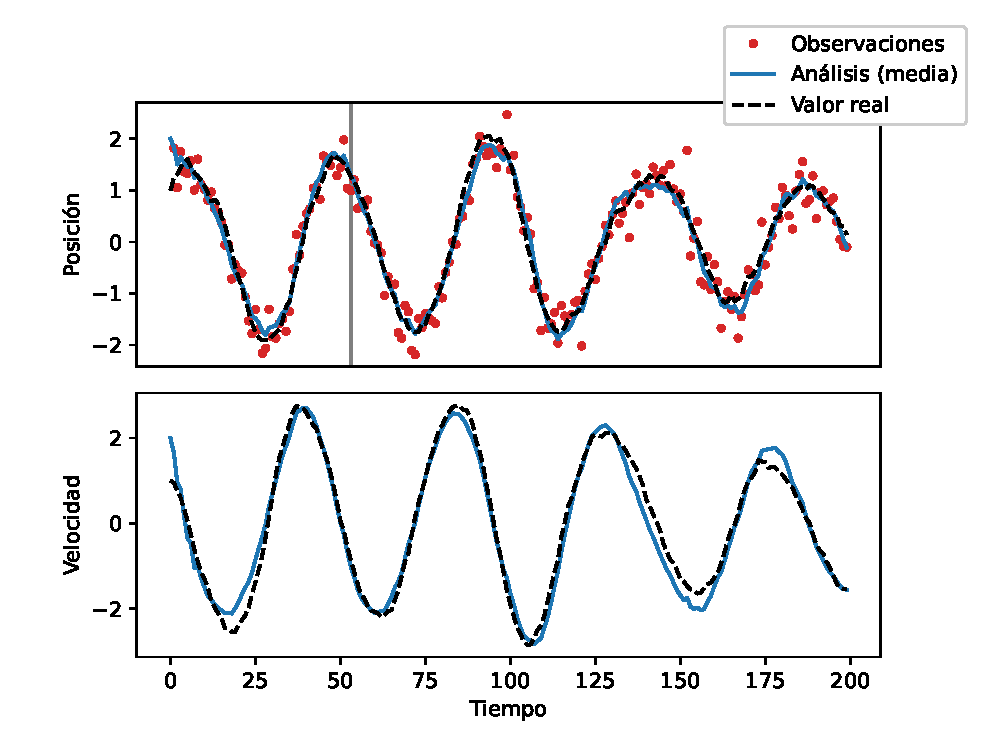
\includegraphics[width=0.75\textwidth]{example_codes/KF_harmonic_oscillator.eps}
    \caption{Trayectorias reales y estimadas mediante el filtro de Kalman. Sólo la posición es observada}
    \label{fig:KF_harmonic_oscillator}
\end{figure}

\begin{figure}[h!]
    \centering
    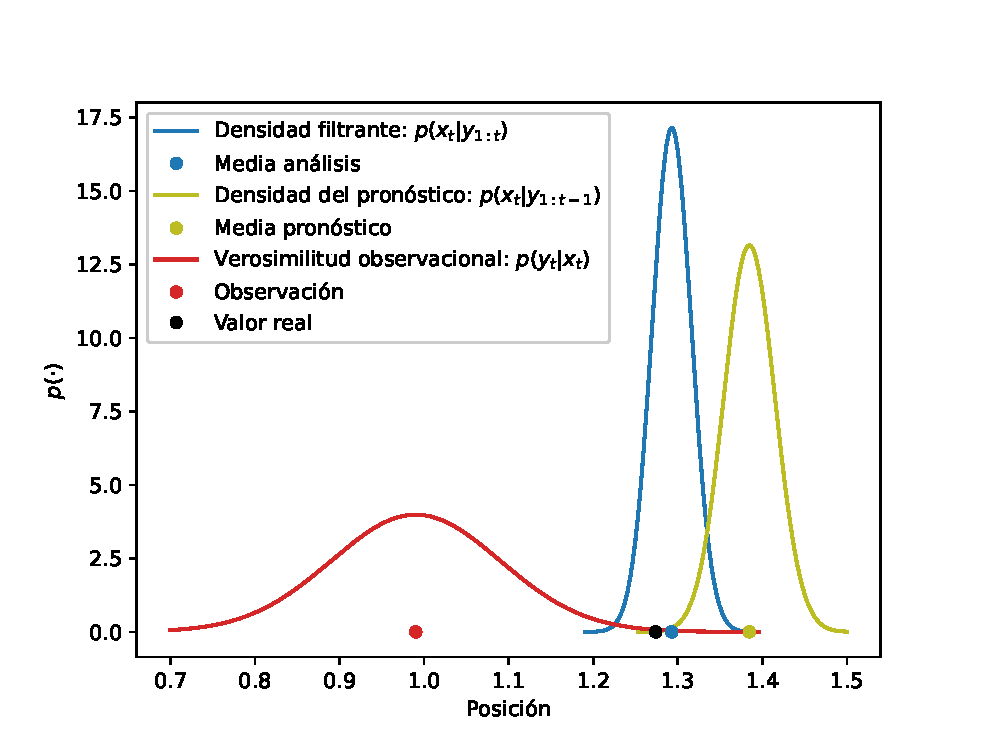
\includegraphics[width=0.75\textwidth]{example_codes/KF_bayes.eps}
    \caption{Funciones de densidad de probabilidad filtrante y de pronóstico junto a la verosimilitud de la observación y el valor real. Corresponde al tiempo indicado por el corte vertical en la figura \ref{fig:KF_harmonic_oscillator}}
    \label{fig:KF_bayes}
\end{figure}

\section{Métodos variacionales}

El problema de obtener un análisis a partir de un pronóstico y una observación puede ser interpretado de manera variacional. Mencionamos brevemente la idea que motiva a los métodos variacionales pues constituyen una familia de técnicas que han sido aplicadas a modelos meteorológicos operacionales y que además dan una perspectiva que enriquece la interpretación de otras estrategias de asimilación de datos. Supongamos que tenemos un pronóstico $\v x^f$ con un error de varianza $\v P^f$ y una observación $\v y$ con un error de varianza $\v R$ y que el operador que mapea el espacio de las variables de estado al espacio de las observaciones se llama $\mathcal{H}$. Si queremos encontrar un valor de análisis $\v x^a$ que minimice el error que introduce el pronóstico y la observación, podemos pensar en minimizar la siguiente función de costo:
\begin{align}
    J(\v x) &= (\v x - \v x^f) {\v P^f}^{-1} (\v x - \v x^f)^T + (\v y - \mathcal{H} (\v x)) \v {R}^{-1} (\v y - \mathcal{H} (\v x))^T \label{eq:3dvar_cost} \\
    &= J^f(\v x) + J^o(\v x)
\end{align}

El primer término da cuenta del costo cuadrático asociado a alejarse del pronóstico y, análogamente, el segundo corresponde a la penalización por alejarse de la observación. Es de esperar entonces que el minimizador de $J$ pondere ambas fuentes de información. De hecho, mientras menor sea el error del pronóstico, mayor será el costo de alejarse de este y para la observación tenemos una situación equivalente. Notemos que esta función de costo supone que los errores sean Gaussianos, aditivos e insesgados. Por otro lado, no hay suposiciones explícitas para el modelo observacional $\mathcal{H}$ y $\mathcal{M}$. De hecho, el modelo de transición ni siquiera está incluído porque se hace la suposición de que ya se cuenta con un pronóstico. Sin embargo, si el pronóstico proviene de un modelo no lineal, no es posible en principio garantizar la Gaussianidad de su error. Sobre el operador observacional también hay que aclarar que dependiendo del método con que se minimice la función de costo, es posible que se necesiten requisitos adicionales: por ejemplo sería esperable que el método de optimización requiera que el operador sea linealizable. En el caso en que este operador sea lineal, $J$ es una función cuadrática con un único mínimo y, de hecho, este coincide con la media del análisis tal como se lo computa en el filtro de Kalman.

La metodología que implementa la minimización de $J$ es comúnmente conocida como 3DVar \citep{Courtier1998}, pero hay que mencionar que el planteo variacional del problema abre la puerta a múltiples variantes, ya que se pueden explorar distintos tipos de optimizadores (por ejemplo simplex, quasi-Newton o gradiente conjugado), distintas condiciones iniciales, precondicionamientos, regularización de $J$, etc. Finalmente mencionamos el método 4DVar \citep{Talagrand1987, Rabier2003} el cual es una extensión de 3DVar pero que procesa una ventana de observaciones simultáneamente, es decir funciona como un suavizador en lugar de como un filtro. El problema que busca optimizar 4DVar es la minimización de una función de costo similar a \ref{eq:3dvar_cost} pero que incluye muchas observaciones. Además se plantea como un problema de optimización con resticciones pues la minimización se hace sujeta a que la solución sea una trayectoria del modelo del que se obtienen los pronósticos.

\section{Técnicas por ensambles}
El filtro de Kalman constituye una técnica robusta que da una solución exacta en el caso de modelos lineales con errores Gaussianos aditivos. En ciertos casos es posible considerar linealizaciónes de los operadores $\mathcal{M}_t$ y $\mathcal{H}_t$ y aplicar el filtro de Kalman tradicional con estas aproximaciones. Este método se denomina filtro de Kalman extendido y también producirá estimaciones de las medias y covarianzas predictivas y filtrantes. Aún así, estas dos técnicas no dan respuesta a dos situaciones frecuentes en las aplicaciones de asimilación de datos. Por un lado, es factible que el modelo no sea linealizabe, ya sea porque es tratado como una caja negra o porque la aproximación lineal es imprecisa. En estas situaciones, los pronósticos serán no Gaussianos y es necesario utilizar técnicas que permitan representar otro tipo de distribuciones. Por otro lado, en modelos meteorológicos es común que el espacio de las observaciones tenga alta dimensionalidad ($\sim 10^5$) y el de las variables de estado aún más ($\sim 10^7$) por lo que computar y almacenar las matrices de covarianza $\v P_t^f$ y $\v P_t^a$ sea prohibitivo \citep{Katzfuss2016}. Para dar cuenta de estos problemas se pueden usar técnicas basadas en partículas o ensambles. Estos, en lugar de representar las distribuciones objetivo a través de sus parámetros como en el filtro de Kalman y el filtro de Kalman extendido, se busca representarlas a través de muestras, es decir un ensamble de puntos en el espacio de las variables de estado. Cada punto muestral suele ser denominado partícula o miembro de ensamble de acuerdo a la técnica en cuestión. Vamos a introducir aquí dos familias de métodos basados en ensambles: los filtros de partículas y los filtros de Kalman por ensambles (EnKFs). Los filtros de partículas permiten, en principio, la representación de distribuciones con formas arbitrarias por lo que pueden ser utilizados en escenarios no Gaussianos. Por otro lado, los EnKFs son habitualmente utilizados para mapear el problema al espacio que generan los miembros del ensamble, el cual tiene una dimensionalidad en general mucho menor que el de las variables de estado haciendo posible el cómputo. Es importante aclarar que ninguna de estas técnicas provee una solución \textit{off-the-shelf} para problemas de asimilación de datos arbitrarios e incluso cada método trae aparejado otro conjunto de dificultades técnicas (por ejemplo la degeneración de pesos en el filtro de partículas o el colapso del ensamble en EnKFs). Tanto para filtros de partículas como EnKFs existe una amplia gama de variaciones e implementaciones que introducen características particulares o que buscan resolver o mitigar algún problema en particular. Comenzaremos introduciendo los filtros de partículas porque estos dan una noción clara de por qué tiene sentido usar muestras para representar distribuciones para luego seguir con los EnKFs.

\subsection{Monte Carlo secuencial}

Los filtros de partículas son también conocidos como métodos de Monte Carlo secuencial ya que utilizan el esquema secuencial de dos pasos de predicción-análisis descrito por las ecuaciones \ref{eq:forward_pred} y \ref{eq:forward_filt}. De hecho, el enfoque de estos métodos es el de resolver las integrales de estas ecuaciones, no de manera explícita sino utlizando las aproximaciones empíricas de las distribuciones implicadas. Si tenemos una función de densidad de probabilidades $p$ y una conjunto de partículas $\{\v x^{(i)}\}_{i=1}^N$ muestreadas de manera independiente con esta probabilidad, i.e. $\v x^{(i)}\sim p$, entonces la aproximación empírica de $p$ basada en esta muestra es:
\begin{align*}
    p(\v x) \approx \frac{1}{N}\sum_{i=1}^N \delta_{\v x^{(i)}}(\v x)
\end{align*}
donde $\delta_{\v a}$ es la delta de Dirac que acumula toda la probabilidad en el punto $\v a$ siendo nula en todo otro punto. Esta aproximación está sustentada en la ley de los grandes números, dado que se pueden aproximar valores esperados en base a la distribución $p$ utilizando la media muestral de las partículas.
\begin{align*}
    \frac{1}{N}\sum_{i=1}^N f(\v x^{(i)}) \xrightarrow{c. s.} \int f(\v x) p(\v x) d \v x
\end{align*}

Existe una generalización de la aproximación de Monte Carlo denominada muestreo de importancia. A pesar de su nombre es un método para aproximar integrales. Cuando no es posible muestrear de $p$ se puede entonces muestrear otra distribución con densidad $q$ que actúe de proxy de $p$. En principio la única condición para $q$ es que su soporte contenga al de $p$. Este método también admite que no se pueda evaluar exactamente $p$ y $q$ sino que sólo podamos evaluar versiones no normalizadas $\tilde{p}$ y $\tilde{q}$ de estas densidades. Entonces, si tenemos un conjunto de partículas $\{\v x^{(i)}\}_{i=1}^N$ tales que $\v x^{(i)}\sim q$, podemos hacer la aproximación dada por las siguientes fórmulas:
\begin{align*}
    \int f(\v x) p(\v x) d \v x &\approx \sum_{i=1}^N w_i f(\v x^{(i)}) \\
    w_i &= \tilde{w}_i / \textstyle\sum_{i=1}^N \tilde{w}_i \\
    \tilde{w}_i &= \tilde{p}(\v x^{(i)}) / \tilde{q}(\v x^{(i)})
\end{align*}
donde $w_i$ son denominados pesos de importancia y $\tilde{w}_i$ son sus versiónes no normalizadas. Por su parte, $q$ es denominada la distribución \textit{propuesta}.

Los métodos de Monte Carlo secuencial producen conjuntos de partículas que aproximan a la distribución filtrante. Estas partícuas además pueden ser ponderadas, es decir pueden traer pesos asociados. Concretamente, para cada tiempo $t$ se obtienen $\{\v x_t^{(i)}, w_t^{(i)}\}_{i=1}^{N}$ tal que sea una aproximación empírica de $p(\v x_t | \v y_{1:t})$.

Los filtros de partículas obtienen estas muestras en dos pasos básicos: primero se muestrean partículas de una distribución propuesta $q$ y luego se computan sus pesos. Con una elección adecuada de $q$ las partículas al tiempo $t$ pueden ser obtenidas a partir de las partículas a tiempo $t-1$ y los pesos pueden ser computados como una actualización de los pesos del tiempo anterior. En particular, dada una muestra pesada $\{\v x_{t-1}^{(i)}, w_{t-1}^{(i)}\}_{i=1}^{N}$ correspondiente al tiempo $t-1$, el procedimiento consiste en:
\begin{itemize}
    \item Muestrear partículas:
        \begin{align*}
            \v x_{t}^{(i)} \sim q(\v x_t | \v x_{t-1}^{(i)}, \v y_t)
        \end{align*}
    \item Actualizar pesos: 
        \begin{align*}
            w_{t}^{(i)} \propto w_{t-1}^{(i)} \frac{p(\v y_t | \v x_t^{(i)}) p(\v x_t^{(i)} | \v x_{t-1}^{(i)})}{q(\v x_t^{(i)} | \v x_{t-1}^{(i)}, \v y_t)}
        \end{align*}
\end{itemize}

Esta implementación es habitualmente llamada SIS (\textit{sequential importance sampling}) y en la práctica tiene el problema de que los pesos suelen concentrarse en una sola partícula, es decir uno de los pesos es prácticamente $1$ mientras que el resto es prácticamente $0$. Este efecto se denomina degeneración del filtro y es indeseable pues la representación muestral de la distribución filtrante pierde expresividad. Además de aumentar el número de partículas existen varias estrategias para mitigar este efecto, la más conocida de ellas es el remuestreo. Este método consiste en muestrar con reemplazo las partículas de la ditribución empirica dada por los pesos. Es decir, una vez computados los pesos se obtiene un nuevo conjunto de partículas con pesos uniformes:
\begin{align*}
    \hat{\v x}_t^{(i)} &\sim \sum_{i=1}^N w_i \delta_{\v x^{(i)}} \\
    \hat{w_i} &= 1 / N
\end{align*}

Esto tiene el efecto que las partículas con mayor peso estarán repetidas y las de menos peso serán eliminadas. A pesar de mitigar la degeneración del filtro causa el problema de empobrecimiento de diversidad del que hablaremos más adelante. No es necesario hacer remuestreo de partículas en cada paso de tiempo y un criterio común para decidir si se hace o no es verificar si el número efectivo de partículas $N_{eff}$ está por debajo de un valor umbral $N_T$. El número efectivo de partículas se puede estimar de la siguiente manera \cite{Arulampalam2002}:
\begin{align*}
    N_{eff} \approx \frac{1}{\sum_{i=1}^N (w_i)^2} \dot{=} \widehat{N_{eff}}
\end{align*}
Este filtro de partículas que incorpora remuestreo suele ser denominado SIR (\textit{sequential importance resampling}) y lo expresamos en forma algortítmica en \ref{algo:sir_pf}.


% TODO: Resolver asignación en algoritmos. Usar := y :~ ?
\begin{algorithm}[H]\label{algo:sir_pf}    
    Muestrear partículas iniciales: $\{\v x_0^{(i)}\}_{i=1}^{N_p} \sim p(\v x_0)$
    
    \For{$t=1, ..., T$}{
        Muestrear partículas de la distribución propuesta: \
        
        \hspace{20pt} $\widehat{\v x}_{t}^{(i)} \sim q(\v x_t | \v x_{t-1}^{(i)}, \v y_t)$ \
        
        Actualizar y normalizar pesos: \
        
        \hspace{20pt} $w_{t}^{(i)} \propto w_{t-1}^{(i)} \frac{p(\v y_t | \widehat{\v x}_t^{(i)}) p(\widehat{\v x}_t^{(i)} | \v x_{t-1}^{(i)})}{q(\widehat{\v x}_t^{(i)} | \v x_{t-1}^{(i)}, \v y_t)}$ \

        Aproximar el número efectivo de partículas: \
        
        \hspace{20pt} $\widehat{N_{eff}} = \frac{1}{\sum_{i=1}^{N_p} (w_i)^2}$ \

        \If{$\widehat{N_{eff}} < N_T$} {
            \begin{flalign*}
                \v x_t^{(i)} &\sim \sum_{i=1}^{N_p} w_i \delta_{\widehat{\v x}_t^{(i)}} & \\
                w_{t}^{(i)} &= 1 / N_p &
            \end{flalign*}            
        }
    }
\caption{Filtro de partículas SIR}
\end{algorithm}

Una de las implementaciones más sencillas de este tipo de filtro es el llamado \textit{bootstrap} y consiste en tomar la distribución propuesta como la probabilidad de transición, i.e., $q(\v x_t | \v x_{t-1}, \v y_t) = p(\v x_t | \v x_{t-1})$. Esto significa que el muestreo de partículas es simpemente aplicar el modelo de transición a todas las partículas del tiempo anterior. Además, las implementaciones más comunes del filtro \textit{bootstrap} hacen remuestreo en cada paso de tiempo. Esto significa que los pesos son sólo calculados para hacer remuestreo pero las partículas que representan a la distribución filtrante tienen pesos uniformes y no hay que almacenarlos. Además esto simplifica el cómputo de los pesos a la expresión $w_{t}^{(i)} \propto p(\v y_t | \v x_t^{(i)})$. En \ref{algo:bootstrap_pf} especificamos este método.

\begin{algorithm}[H]\label{algo:bootstrap_pf}
    Muestrear partículas iniciales: $\{\v x_0^{a, (i)}\}_{i=1}^{N_p} \sim p(\v x_0)$
    
    \For{$t=1, ..., T$}{
        Evolucionar partículas: \
        
        \hspace{20pt} $\v x_{t}^{f, (i)} \sim p(\v x_t | \v x_{t-1}^{a, (i)})$  para $i = 1, ..., N_p$ \
        
        Actualizar y normalizar pesos: \
        
        \hspace{20pt} $w^{(i)} \propto p(\v y_t | \v x_t^{f, (i)})$ \
        
        Remuestrear: \
        
        \hspace{20pt} $\v x_t^{a, (i)} \sim \sum_{i=1}^{N_p} w_i \delta_{\v x^{f, (i)}}$
        }
\caption{Filtro de partículas bootstrap}
\end{algorithm}

La elección de la distribución de transición como distribución propuesta en el filtro de partículas \textit{bootstrap} significa que el muestreo de partículas no es más que evolucionar cada partícula del tiempo anterior utilizando el modelo. Las partículas muestradas constituyen entonces un pronóstico. Esta interpretación no es generalizable al filtro SIR general. Para indicar esto en \ref{algo:bootstrap_pf} usamos el supraíndice $f$ (por \textit{forecast}) en las partículas del pronóstico y $a$ en las de análisis. 

El cómputo de los pesos está dado por la verosimilitud observacional por lo que estos cuantifican cuán afín es cada partícula a la observación. Por su parte, la forma de transformar al conjunto de partículas de pronóstico en una muestra filtrante es a través de el remuestreo. El remuestreo, al ser con reemplazo, tiene el efecto de multiplicar las partículas con pesos altos (cercanas a la observación) y eliminar las partículas con pesos bajos (lejanas a la observación). Este mecanismo se suele comparar con la selección natural, sólo sobreviven y se reproducen las partículas ``más aptas''.

Como se anticipó, el remuestreo introduce otro problema: el empobrecimiento de diversidad. Esto se debe a que tendremos muchas réplicas de las partículas con más peso, es decir una muestra que cubre pobremente el espacio muestral. Este efecto es claramente indeseable y para paliarlo es habitual introducir, luego del remuestreo, un paso en el que las partículas se mutan o se mueven de alguna forma para no tener tantas partículas repetidas. El término mutación proviene de la interpretación del fitro de partículas \textit{bootstrap} como un mecanismo de selección del más apto. Esta modificación de las partículas se puede hacer incorporando pasos de MCMC. También es posible mitigar el problema mediante regularización, utilizando \textit{kernel density estimation} sobre las distribuciones empíricas \citep{Sarkka2013, Arulampalam2002, Ruchi2019}.
% TODO: introducir sin mucho detalle filtros de flujo de langevin y VMPF

La diversidad de filtros de partículas es vasta: la transformación de un conjunto de partículas que representa un pronóstico en una muestra de la probabilidad \textit{a posteriori} puede ser lograda con diversos enfoques. Existen combinaciones con ideas de filtros de Kalman, filtros que utilizan ideas de transporte óptimo para mover las partículas hacia la distribución deseada, temperado de la verosimilitud para evitar pesos muy pequeños cuando esta es muy concentrada o filtros que mueven dinámicamente las partículas mediante un flujo hacia la distribución \textit{a posteriori}. En \cite{vanLeeuwen2019} se puede encontrar un buen reporte sobre las diversas implementaciones de filtros de partículas. 

% TODO: mejorar este párrafo de ventajas y desventajas de PFs en general
El filtro de partículas SIR tiene la ventaja de hacer pocos requisitos sobre el modelo. En el caso particular del filtro \textit{bootstrap} sólo se necesita evaluar la verosimilitud observacional y muestrear de la probabilidad de transición. Obtener muestra de la probabilidad de transición no es otra cosa que evolucionar el modelo, y este requisito por sí solo significa que el modelo puede ser tratado como una caja negra, una característica deseable en muchas situaciones. Como no hay ninguna suposición sobre las distribuciones, estos métodos pueden ser utilizados en escenarios de no-Gaussianidad y no-linealidad. Por otro lado, este tipo de filtros habitualmente necesitan muchas partículas para tener una buena performance y además padecen de los problemas ya mencionados de degeneración del fitro y empobrecimiento de la diversidad. También es común que muchos pesos sean muy pequeños, lo cual puede causar problemas numéricos. Estos problemas se acentúan en espacios de alta dimensionalidad por lo que en estas situaciones es habitual utilizar filtros de Kalman por ensambles, los cuales introducimos más adelante.

\subsubsection{VMPF}

En el trabajo de investigación de esta tesis utilizamos un filtro basado en flujo de partículas llamado filtro de partículas de mapeo variacional (VMPF, \cite{Pulido2019}), para utilizar en combinación con las técnicas de tratamiento de errores observacionales y de modelo desarrolladas. Hacemos una breve mención sobre la idea que sobyace a este método. En los filtros basados en flujo de partículas se considera que estas obedecen en un pseudotiempo $s$ a una ecuación diferencial
\begin{align*}
    \frac{d\v x}{ds} = f_s(\v x)
\end{align*}
de manera que las partículas en el pseudotiempo inicial se distribuyen como la \textit{prior} y en el pseudotiempo final obedecen a la distribución \textit{a posteriori} pasando por distribuciones intermedias $p_s$. En particular, el VMPF mueve las partículas en la dirección de máximo decenso del gradiente de la divergencia de Kullback-Leibler entre $p_s$ y la distribución objetivo. Además, para evaluar el este gradiente se considera una versión kernelizada de la divergencia de Kullback-Leibler. Esto resulta en que, discretizando el pseudotiempo, tenemos:
\begin{align*}
    \v x_{s+1} &= \v x_s - \epsilon \nabla KL(\v x_s) \\
    &= \v x_s - \epsilon \int p_s(\v z) (K(\v z, \v x_s) \nabla_{\v z} log(\v z | \v y) + \nabla_{\v z} K(\v z, \v x_s)) d\v z
\end{align*}
donde $K$ es el kernel y la integral que representa al gradiente puede ser aproximado utilizando Monte Carlo utilizando la muestra de partículas de la distribución $p_s(\v z)$ disponible de la iteración correspondiente a pseudotiempo anterior. El método resultante tiene la cualidad de que las partículas se mueven hacia la moda de la distribución $p(\v x | \v y)$ pero la amplitud de banda del kernel actúa como una fuerza repulsiva entre las partículas \citep{Liu2016} de manera que la muestra resultante no pierde diversidad. Al utilizar una única partícula esta se dirige a la moda de la distribución objetivo, dando la estimación MAP (máximo \textit{a posteriori}) la cual, notablemente, es la que se obtiene mediante métodos variacionales como el 3DVAR.

\subsection{EnKF} \label{sec:enkf}

Los filtros de Kalman por ensambles utilizan muestras para mantener estimaciones de las distribuciones objetivo pero incorporan las fórmulas del filtro de Kalman tradicional para actualizar las partículas (en el contexto del EnKF las partículas suelen ser llamadas miembros del ensamble pero utilizaremos las terminologías de manera intercambiable). Para esto es necesario suponer linealidad sobre el modelo de transición y observacional y también errores aditivos Gaussianos: es decir que trabaja sobre el modelo definido por \ref{eq:kf_forward} y \ref{eq:kf_observational}. En realidad, la suposición de que el modelo de transición es lineal puede ser algo relajada en la práctica pero discutiremos esto más adelante.

Supongamos que a tiempo $t-1$ contamos con un ensamble $\{ \v x_{t-1}^{a, (i)} \}_{i=1}^{N_p}$ que representa al análisis. Por las suposiciones que hemos hecho esta muestra será Gaussiana y al aplicar el modelo transicional sobre cada uno de estos miembros del ensamble podemos obtener un ensamble $\{ \v x_{t}^{f, (i)} \}_{i=1}^{N_p}$ del pronóstico a tiempo $t$ el cual constutuirá una muestra Gaussiana. La pregunta entonces, es cómo obtener a partir de este ensamble otro que represente al análisis. La idea de el EnKF es aplicar la ecuación de actualización de la media del filtro de Kalman tradicional \ref{eq:kf_mean_filter} para cada partícula del pronóstico. Esta es la esencia de los EnKF pero para aplicar el concepto correctamente debemos hacer algunas salvedades.

Para aplicar la actualización del filtro de Kalman ecesitamos computar $\v K_t$ la cual por su parte necesita de la matriz de covarianzas del pronóstico $\v P_t^f$. Sin embargo, a diferencia del filtro de Kalman, aquí no propagamos las matrices de covarianzas en el tiempo, sólo una muestra de la distribución y por ello no disponemos de una representación exacta de esta. De cualquier manera, es natural aproximar $\v P_t^f$ con la matriz de covarianza muestral del ensamble del pronóstico, $\widehat{\v P}_t^f$ para obtener una aproximación $\widehat{\v K}_t$ de la matriz de ganancia de Kalman.

Por otro lado, hay que notar que estamos utilizando sobre cada partícula la fórmula de actualización de la media de la distribución, y cada partícula está siendo actualizada en base a la misma observación. Es posible demostrar que si hacemos esto, la covarianza del ensamble del análisis va a estar subestimada. La solución a este problema consiste en actualizar cada partícula usando una perturbación de la observación original. Para obtener el miembro del ensamble $\v x_t^{a, (i)}$ utilizaremos la observación modificada $\v y_t^{(i)} = \v y_t + \v v_t^{(i)}$ con $\v v_t{(i)} \sim \mathcal{N}(\v 0, \v R_t)$. El origen de este problema y su solución son planteados en \cite{Burgers1998}. El método resultante es denominado EnKF estocástico o EnKF con observaciones perturbadas y en \ref{algo:enkf_pert_obs} está descrito de manera algorítmica. En \ref{appendix:enkf} demostramos que la formulación de este método es correcta.

\begin{algorithm}[H]\label{algo:enkf_pert_obs}
    Muestrear ensamble inicial: $\{\v x_0^{a, (i)} \}_{i=1}^{N_p} \sim p(\v x_0)$
    
    \For{$t=1, ..., T$}{
        \For{$i=1, ..., N_p$} {
            $\gv\eta^{(i)} \sim \mathcal{N}(\v 0, \v Q_t)$ \

            $\v x_t^{f, (i)} = \mathcal{M}_t (\v x_{t-1}^{a, (i)}) + \gv\eta^{(i)}$ \
        }

        % Computar $\widehat{\v P}_t^f$, la covarianza muestral de $\{ \v x_t^{f, (i)} \}_{i=1}^{N_p}$ \

        $\widehat{\v x}_t^f = \frac{1}{N_p}\sum_{i=1}^{N_p} \v x_t^{f, (i)}$ \

        $\widehat{\v P}_t^f = \frac{1}{N_p-1}\sum_{i=1}^{N_p} (\v x_t^{f, (i)} - \widehat{\v x}_t^{f}) (\v x_t^{f, (i)} - \widehat{\v x}_t^{f})^T$ \

        $\widehat{\v K}_t = \widehat{\v P}_t^f \v H_t^T(\v R_t + \v H_t \widehat{\v P}_t^f \v H_t^T)^{-1}$ \

        \For{$i=1, ..., N_p$} {
            $ \v v^{(i)} \sim \mathcal{N}(\v 0, \v R_t)$ \

            $ \v y_t^{(i)} = \v y_t + \v v^{(i)} $ \

            $\v x_t^{a, (i)} = \v x_t^{f, (i)} + \widehat{\v K}_t (\v y_t^{(i)} - \v H_t \v x_t^{f, (i)})$ \
        }

    }
\caption{EnKF estocástico}
\end{algorithm}

Notemos que la suposición de que el modelo de transición es lineal es la suposición que permite asumir que evolucionar los miembros del ensamble hacia adelante va a conservar la Gaussianidad de la muestra. Sin embargo, a diferencia del filtro de Kalman tradicional, no precisamos una expresión matricial $\v M_t$ del operador. El modelo se usa solamente para propagar las partículas hacia adelante por lo cual podemos relajar la hipótesis de linealidad y pensar en un operador general $\mathcal{M}_t$ que si es levemente no lineal podrá preservar la Gaussianidad en los pronósticos y que además puede ser tratado como una caja negra. De hecho, el EnKF es habitualmente presentado como un método apto para modelos no lineales.

Además del filtro, existe la posibilidad de obtener representaciones de ensambles de las distribuciones suavizantes utilizando el llamado suavizador de Kalman por ensambles (EnKS). Así como el EnKF se basa en los pasos de predicción y análisis del pase hacia adelante del algoritmo \textit{forward-backward}, la versión del EnKS conocida como Rauch-Tung-Striebel (RTS) consiste en un pase hacia atrás. En el algoritmo \ref{algo:enks} muestra el método como es sugerido en \cite{Cosme2012}. Notablemente, la metodología se vale solamente de los ensambles de pronóstico y filtrantes producidos por el EnKF por lo que no se necesitan evaluaciones del modelo o del operador observacional. Las partículas suavizantes a tiempo $t$ son computadas como una corrección de las del análisis en las que se incorpora secuencialmente la información de los ensambles aa tiempo $t+1$ mediante la pondereación de una matriz de ganancia $\v K_t^s$. Esta ganancia se computa utilizando $\v S_t^a$ y $\v S_{t+1}^f$ las cuales son matrices cuyas columnas son los miembros de los ensambles $\{\v x_{t+1}^{f, (i)}\}_{t=1}^{N_p}$ y  $\{\v x_t^{a, (i)}\}_{t=1}^{N_p}$ respectivamente, centrados en su media.

\begin{algorithm}[H]\label{algo:enks}
    Definir: $\{\v x_T^{s, (i)} \}_{i=1}^{N_p} = \{\v x_T^{a, (i)} \}_{i=1}^{N_p}$
    
    \For{$t=T-1, ..., 1$}{
        $\v K_t^s = \v S_t^a ((\v S_{t+1}^f)^T \v S_{t+1}^f)^{-1}(\v S_{t+1}^f)^T$ \\
        \For{$i=1, ..., N_p$} {
            $\v x_t^{s, (i)} = \v x_t^{a, (i)} + \v K_t^s (\v x_{t+1}^{s, (i)} - \v x_{t+1}^{f, (i)})$
        }
    }
\caption{RTS EnKS}
\end{algorithm}

% TODO: mejorar este párrafo?
El EnKF que presentamos es solamente una implementación sencilla de esta idea pero la realidad es que existe una gran familia de filtros de Kalman por ensambles desarrollados para diferentes tipos de problemas. Los filtros de raíz cuadrada (EnSRF) y los filtros de Kalman por ensambles ajustados (EAKF) sortean necesidad de perturbar las observaciones, lo cual puede causar subestimación de covarianzas \citep{Whitaker2002, Anderson2001}. Los filtros transformados (ETKF) operan sobre el espacio generado por lso miembros del ensamble y consiguen una mejor eficiencia \citep{Bishop2001}.

En general, los EnKFs son métodos robustos, relativamente fáciles de comprender e implementar y que han sido utilizados en una amplia variedad de problemas. Debido a su popularidad, existen muchas modificaciones para mitigar los problemas más comunes que suele presentar. Los EnKF son especialmente aptos para problemas de gran dimensionalidad ya que pueden representar distribuciones en este tipo de espacios con una cantidad relativamente chica de miembros de ensamble. Además, se pueden optimizar numéricamente y tienen potencial para ser implementados de manera paralela. A pesar de que pueden fallar en modelos altamente no lineales que resulten en pronósticos no Gaussianos, en general pueden dar buena performance incluso en presencia de no linealidades. Esta familia de filtros ha disputado con la técnica variacional 4DVAR como método de asimilación de datos operacional en predicción meteorológica numérica.

\paragraph{Inflación y localización} \

Los EnKFs son utilizados en escenarios de alta dimensionalidad en los que surgen una variedad de problemas. Por un lado, debido a que la cantidad de miembros de ensamble resulta pequeña en comparación con la dimensión de las variables de estado, el error de muestreo asociado puede resultar en que la matriz de covarianza predictiva $\widehat{\v P}_t^f$ esté subestimada o que tenga deficiencias de rango \citep{Miyoshi2011}. Esta situación puede estar incluso profundizada por una mala especificación del error de modelo. Esto puede provocar que la dispersión del ensamble sea muy compacta (esto se suele llamar colapso del ensambles) lo cual da como resultado que la certidumbre sobre la predicción sea mayor de lo que debería ser y por lo tanto la información observacional sea menos considerada por el sistema de asimilación de datos. Como resultado, es posible que el filtro comienze a ignorar las observaciones y diverja de la trayectoria que debería estimar. Un paliativo a esta situación es la llamada inflación de covarianza que consiste en agrandar artificialmente la covarianza predictiva \citep{Anderson1999}. Existen diversas implementaciones de esta idea pero distinguimos la inflación aditiva que consiste en añadir ruido a los miembros del ensamble y la inflación multiplicativa que en general es implementada multiplicando la matriz de covarianzas (o las desviaciones de los miembros del ensamble respecto a su media) por un escalar mayor a $1$. Para mejorar la calidad de la matriz de covarianzas predictiva, además se suele usar localización. Esta metodología consiste en reducir el valor de los términos fuera de la diagonal que correspondan a covarianzas de variables lejanas espacialmente y que por lo tanto no deberían estar muy correlacionadas. Esto se hace porque un número bajo de miembros de ensamble puede provocar correlaciones espúreas que deterioren la calidad de la matriz de covarianzas \citep{Hamill2001}. Utilizando localización se puede mitigar la deficiencia de rango y el error de muestreo. 
